%!TeX program = xelatex
\documentclass[12pt,hyperref,a4paper,UTF8]{ctexart}

\usepackage{SJTUReport}
\usepackage{float}
\usepackage{booktabs}
\usepackage{multirow}
\usepackage{geometry}
\usepackage{array}
\usepackage{graphicx}
\usepackage{amsmath}
\usepackage{amssymb}
\usepackage{siunitx}
\usepackage{longtable}
\usepackage{enumitem}
\usepackage{caption}
\usepackage{xcolor}
\usepackage{bm}
\usepackage{listings}
\usepackage{tikz}
\usetikzlibrary{arrows.meta, positioning, shapes.geometric, fit, backgrounds}

\geometry{a4paper, margin=1in}

%% ---- 课程信息覆盖 ----
\fancyhead[L]{\fangsong 通用及图形处理器架构与系统}

\title{
    \vspace{3cm}
    \heiti \Huge \textbf{{通用及图形处理器架构与系统课程报告}} \par
    \vspace{1cm}
    \heiti \Large {\underline{LAB：RISC-V 处理器设计与实现}}
    \vspace{3cm}
}

\author{
    \vspace{0.5cm}
    \kaishu\Large 学院\ \dlmu[9cm]{集成电路学院} \\
    \vspace{0.5cm}
    \kaishu\Large 邮箱\ \dlmu[9cm]{yuri\_cang@sjtu.edu.cn} \\
    \vspace{0.5cm}
    \kaishu\Large 学号\ \dlmu[9cm]{523031910352} \qquad \\
    \vspace{0.5cm}
    \kaishu\Large 姓名\ \dlmu[9cm]{方兴宇} \qquad \\
}

\date{\today}

%% ---- Verilog 代码样式 ----
\lstdefinelanguage{Verilog}{
    morekeywords={module, endmodule, input, output, inout, wire, reg,
                  always, assign, begin, end, if, else, case, endcase,
                  posedge, negedge, parameter, integer, for, localparam,
                  initial, forever, timescale},
    sensitive=true,
    morecomment=[l]{//},
    morecomment=[s]{/*}{*/},
    morestring=[b]"
}
\lstset{
    language=Verilog,
    basicstyle=\small\ttfamily,
    keywordstyle=\color{blue!80!black}\bfseries,
    commentstyle=\color{gray}\itshape,
    stringstyle=\color{red!70!black},
    numberstyle=\tiny\color{gray},
    numbers=left,
    numbersep=6pt,
    breaklines=true,
    frame=single,
    framerule=0.4pt,
    tabsize=4,
    showstringspaces=false,
    captionpos=b,
    xleftmargin=2em,
}

% -------------------------------------------------------
\begin{document}

\cover
\tableofcontents
\newpage

% =======================================================
\section{实验目的}
% =======================================================

本实验基于 RISC-V 精简指令集架构，使用 Verilog HDL 完成两类处理器的设计与验证，具体目标如下：

\begin{enumerate}[leftmargin=2em]
    \item 掌握 RISC-V 32 位整数基础指令集（RV32I）的编码规则与执行语义，理解 R/I/S/B/J 五种指令格式；
    \item 实现支持 13 条基础指令的\textbf{单周期}处理器，建立五阶段数据通路（IF--ID--EX--MEM--WB）的基本概念；
    \item 在单周期代码备份的基础上，通过在各级之间插入时序触发器（Flip-Flop）将数据通路改造为\textbf{五级流水线}结构，提升吞吐量；
    \item 分析并解决流水线中的\textbf{数据冲突}（Data Hazard）与\textbf{控制冲突}（Control Hazard），实现数据转发（Forwarding）与流水线阻塞（Stall）机制；
    \item 通过功能仿真验证两种处理器实现的正确性，使用提供的自动化测试工具通过全部 13 条指令测试用例。
\end{enumerate}

% =======================================================
\section{实验原理}
% =======================================================

\subsection{RISC-V 指令集子集}

本实验实现 RV32I 中的 13 条指令，涵盖算术、逻辑、移位、访存、分支和跳转六类，详见\autoref{tab:isa}。

\begin{table}[H]
    \centering
    \caption{实现的 13 条 RISC-V 指令}
    \label{tab:isa}
    \begin{tabular}{>{\centering}p{1.6cm} >{\centering}p{1.2cm} c >{\centering}p{4.5cm} c}
        \toprule
        类别 & 指令 & 格式 & 功能描述 & ALU 操作码 \\
        \midrule
        \multirow{3}{*}{算术} & ADD  & R & $\text{rd} = \text{rs1} + \text{rs2}$ & 4'd0 \\
                               & ADDI & I & $\text{rd} = \text{rs1} + \text{imm}$ & 4'd0 \\
                               & SUB  & R & $\text{rd} = \text{rs1} - \text{rs2}$ & 4'd1 \\
        \midrule
        \multirow{3}{*}{逻辑} & AND  & R & $\text{rd} = \text{rs1}~\&~\text{rs2}$  & 4'd2 \\
                               & OR   & R & $\text{rd} = \text{rs1}~|~\text{rs2}$  & 4'd3 \\
                               & XOR  & R & $\text{rd} = \text{rs1}~\hat{}~\text{rs2}$ & 4'd4 \\
        \midrule
        \multirow{2}{*}{移位} & SLL  & R & $\text{rd} = \text{rs1} \ll \text{rs2}[4:0]$ & 4'd5 \\
                               & SRL  & R & $\text{rd} = \text{rs1} \gg \text{rs2}[4:0]$ & 4'd6 \\
        \midrule
        \multirow{2}{*}{访存} & LW   & I & $\text{rd} = \text{Mem}[\text{rs1}+\text{imm}]$ & 4'd0 \\
                               & SW   & S & $\text{Mem}[\text{rs1}+\text{imm}] = \text{rs2}$ & 4'd0 \\
        \midrule
        \multirow{2}{*}{分支} & BEQ  & B & if (rs1==rs2) PC$\mathrel{+}=$imm & 4'd1 \\
                               & BLT  & B & if (rs1$<$rs2) PC$\mathrel{+}=$imm（有符号） & 4'd1 \\
        \midrule
        跳转 & JAL  & J & $\text{rd}=\text{PC}+4;\ \text{PC}\mathrel{+}=\text{imm}$ & 4'd0 \\
        \bottomrule
    \end{tabular}
\end{table}

RISC-V 所有指令均为 32 位定长编码。立即数编码方式随指令格式不同而变化，\autoref{tab:imm}归纳了五种立即数的位域拼接规则。

\begin{table}[H]
    \centering
    \caption{RISC-V 立即数编码规则}
    \label{tab:imm}
    \begin{tabular}{lll}
        \toprule
        类型 & 拼接来源（inst 字段） & 用途 \\
        \midrule
        I 型 & \{inst[31:20]\}，符号扩展至 32 位 & ADDI、LW 等 \\
        S 型 & \{inst[31:25], inst[11:7]\}，符号扩展 & SW \\
        B 型 & \{inst[31], inst[7], inst[30:25], inst[11:8], 1'b0\}，符号扩展 & BEQ、BLT \\
        U 型 & \{inst[31:12], 12'b0\} & LUI、AUIPC \\
        J 型 & \{inst[31], inst[19:12], inst[20], inst[30:21], 1'b0\}，符号扩展 & JAL \\
        \bottomrule
    \end{tabular}
\end{table}

\subsection{单周期处理器}

单周期处理器每个时钟周期完成一条指令的取指、译码、执行、访存与写回全部操作。五个功能模块之间通过组合逻辑信号直接相连，无寄存器打拍，如\autoref{fig:single_dp}所示：

\begin{figure}[H]
\centering
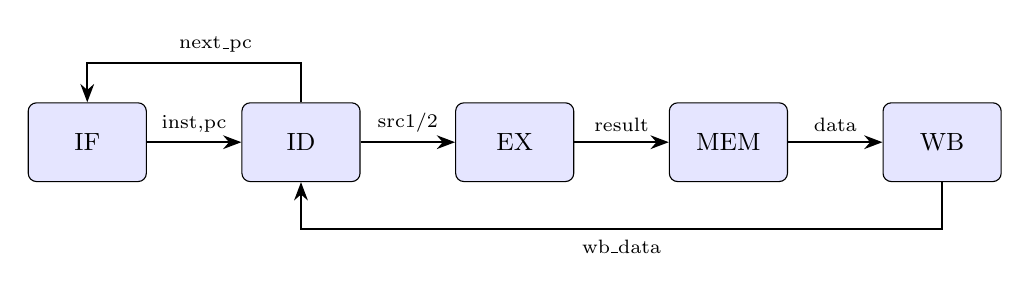
\begin{tikzpicture}[
    stage/.style={draw, minimum width=1.5cm, minimum height=1cm,
                  fill=blue!10, rounded corners=3pt, align=center, font=\small},
    arr/.style={-Stealth, thick}
]
\node[stage] (IF)  {IF};
\node[stage, right=1.2cm of IF]  (ID)  {ID};
\node[stage, right=1.2cm of ID]  (EX)  {EX};
\node[stage, right=1.2cm of EX]  (MEM) {MEM};
\node[stage, right=1.2cm of MEM] (WB)  {WB};

\draw[arr] (IF) -- node[above,font=\scriptsize]{inst,pc} (ID);
\draw[arr] (ID) -- node[above,font=\scriptsize]{src1/2} (EX);
\draw[arr] (EX) -- node[above,font=\scriptsize]{result} (MEM);
\draw[arr] (MEM)-- node[above,font=\scriptsize]{data} (WB);

% WB回写
\draw[arr] (WB.south) -- ++(0,-0.6) -| node[below,font=\scriptsize,pos=0.25]{wb\_data} (ID.south);

% 分支
\draw[arr] (ID.north) -- ++(0,0.5) -| node[above,font=\scriptsize,pos=0.2]{next\_pc} (IF.north);
\end{tikzpicture}
\caption{单周期处理器数据通路}
\label{fig:single_dp}
\end{figure}

\subsection{五级流水线处理器}

流水线处理器在相邻阶段间插入\textbf{流水线寄存器}（时序触发器），使不同指令的各阶段可以在不同周期同时执行，理论峰值吞吐量接近每周期一条指令（IPC = 1）。\autoref{tab:pipe_timing}展示了五级流水线的时空关系：

\begin{table}[H]
    \centering
    \caption{五级流水线时空图（4 条指令示例）}
    \label{tab:pipe_timing}
    \begin{tabular}{lcccccccc}
        \toprule
        指令 & C1 & C2 & C3 & C4 & C5 & C6 & C7 & C8 \\
        \midrule
        I1 & \textbf{IF} & ID & EX & MEM & WB & & & \\
        I2 & & \textbf{IF} & ID & EX & MEM & WB & & \\
        I3 & & & \textbf{IF} & ID & EX & MEM & WB & \\
        I4 & & & & \textbf{IF} & ID & EX & MEM & WB \\
        \bottomrule
    \end{tabular}
\end{table}

\subsubsection{数据冲突（Data Hazard）}

当后续指令的源操作数依赖前序指令尚未写回的结果时，发生写后读（RAW）数据冲突。按距离分三类：

\begin{itemize}[leftmargin=2em]
    \item \textbf{距离 1 拍}（生产者在 EX/MEM）：通过 EX/MEM$\rightarrow$EX 转发，零延迟解决；
    \item \textbf{距离 2 拍}（生产者在 MEM/WB）：通过 MEM/WB$\rightarrow$EX 转发，零延迟解决；
    \item \textbf{距离 3 拍}（WB 写与 ID 读同周期）：通过寄存器堆\textbf{写优先}（WB$\rightarrow$ID）转发，零延迟解决；
    \item \textbf{Load-Use 冲突}（LW 后紧接使用）：数据在 MEM 阶段末才就绪，无法纯转发，需\textbf{阻塞 1 拍}，再由 MEM/WB$\rightarrow$EX 转发提供数据。
\end{itemize}

\subsubsection{控制冲突（Control Hazard）}

BEQ、BLT、JAL 在 ID 阶段确定跳转目标，而此时 IF 阶段已取入了顺序下一条（错误路径）指令。解决方案：检测到跳转时\textbf{冲刷}（Flush）IF/ID 寄存器（置零 = 插入 NOP），代价为 1 个时钟周期损失。

% =======================================================
\section{处理器设计与实现}
% =======================================================

\subsection{模块层次与接口}

SoC 的模块例化层次如\autoref{tab:hierarchy}所示，\texttt{riscv\_soc\_tb.v}、\texttt{inst\_mem.v}、\texttt{data\_mem.v} 由实验框架提供，接口固定不可修改；\texttt{riscv.v} 及内部所有子模块由本实验自行实现。

\begin{table}[H]
    \centering
    \caption{模块层次结构}
    \label{tab:hierarchy}
    \begin{tabular}{lll}
        \toprule
        模块名 & 文件 & 功能 \\
        \midrule
        \texttt{riscv\_soc\_tb} & \texttt{riscv\_soc\_tb.v} & 仿真顶层，产生时钟/复位，例化三个子模块 \\
        \quad\texttt{riscv} & \texttt{riscv.v} & \textbf{处理器顶层}（接口不可更改） \\
        \quad\quad\texttt{if\_stage} & \texttt{if.v} & 取指：维护 PC 寄存器 \\
        \quad\quad\texttt{id\_stage} & \texttt{id.v} & 译码：指令解析、立即数扩展、控制信号生成 \\
        \quad\quad\texttt{ex\_stage} & \texttt{ex.v} & 执行：7 种 ALU 运算 \\
        \quad\quad\texttt{mem\_stage} & \texttt{men.v} & 访存：地址/数据整理，驱动外部存储器接口 \\
        \quad\quad\texttt{register} & \texttt{register.v} & 32 个通用寄存器堆（x0 恒为 0） \\
        \quad\texttt{inst\_mem} & \texttt{inst\_mem.v} & 指令存储器，从 \texttt{machinecode.txt} 加载 \\
        \quad\texttt{data\_mem} & \texttt{data\_mem.v} & 数据存储器，含 \texttt{verify} 验证输出 \\
        \bottomrule
    \end{tabular}
\end{table}

处理器顶层对外接口遵循实验规范，如\autoref{tab:riscv_ports}所示。

\begin{table}[H]
    \centering
    \caption{\texttt{riscv.v} 顶层接口定义}
    \label{tab:riscv_ports}
    \begin{tabular}{llcl}
        \toprule
        信号名 & 方向 & 位宽 & 描述 \\
        \midrule
        \texttt{clk}          & input  & 1  & 时钟信号 \\
        \texttt{rst}          & input  & 1  & 复位（高有效） \\
        \texttt{inst\_i}      & input  & 32 & 从指令存储器读入的指令 \\
        \texttt{inst\_addr\_o}& output & 32 & 当前 PC（指令存储器地址） \\
        \texttt{inst\_ce\_o}  & output & 1  & 指令存储器使能 \\
        \texttt{data\_i}      & input  & 32 & 从数据存储器读入的数据 \\
        \texttt{data\_we\_o}  & output & 4  & 写使能（字节掩码，全 0 为读） \\
        \texttt{data\_ce\_o}  & output & 1  & 数据存储器使能 \\
        \texttt{data\_addr\_o}& output & 32 & 数据存储器地址 \\
        \texttt{data\_o}      & output & 32 & 写入数据存储器的数据 \\
        \bottomrule
    \end{tabular}
\end{table}

\subsection{单周期处理器实现（single/）}

\subsubsection{IF 阶段（\texttt{if\_stage}）}

IF 阶段维护 PC 寄存器，每周期输出当前 PC 并驱动指令存储器取指。PC 的更新逻辑如下：复位时清零，检测到分支/跳转时（\texttt{pc\_we}=1）载入目标地址，否则顺序加 4。

\begin{lstlisting}[caption={if\_stage PC 更新逻辑}]
always @(posedge clk or posedge rst) begin
    if (rst)        pc <= 32'b0;
    else if (pc_we) pc <= next_pc;  // 分支/跳转
    else            pc <= pc + 4;   // 顺序执行
end
\end{lstlisting}

\subsubsection{ID 阶段（\texttt{id\_stage}）}

ID 阶段完成指令的全部译码工作，包括：
\begin{itemize}[leftmargin=2em]
    \item 字段解析：opcode[6:0]、funct3[14:12]、funct7[31:25]、rs1/rs2/rd 地址；
    \item 立即数扩展：根据指令格式对 I/S/B/J 型立即数进行符号扩展；
    \item 控制信号生成：\texttt{alu\_op}、\texttt{src2\_sel}、\texttt{reg\_we}、\texttt{mem\_ce}、\texttt{mem\_we}；
    \item 分支条件求值：BEQ/BLT 直接在 ID 阶段比较 rdata1/rdata2，输出 \texttt{pc\_we} 和 \texttt{next\_pc}，单周期下无延迟损失。
\end{itemize}

操作数来源由 \texttt{src2\_sel} 信号控制：0 = rs2 寄存器值（R 型），1 = 立即数（I/S 型），2 = 保留，3 = 常数 4（JAL 返回地址）。对于 JAL，还需 \texttt{src1\_sel}=1 以在 EX 阶段选择 PC 而非寄存器值。

\subsubsection{EX 阶段（\texttt{ex\_stage}）}

EX 阶段为纯组合逻辑 ALU，支持 7 种运算：

\begin{lstlisting}[caption={ALU 运算实现}]
case (alu_op)
    4'd0: alu_result = src1 + src2;          // ADD/ADDI/LW/SW/JAL
    4'd1: alu_result = src1 - src2;          // SUB
    4'd2: alu_result = src1 & src2;          // AND
    4'd3: alu_result = src1 | src2;          // OR
    4'd4: alu_result = src1 ^ src2;          // XOR
    4'd5: alu_result = src1 << src2[4:0];   // SLL
    4'd6: alu_result = src1 >> src2[4:0];   // SRL
    default: alu_result = 32'b0;
endcase
\end{lstlisting}

LW 和 SW 的地址均通过 ALU 加法计算（$\text{rs1} + \text{imm}$）；BEQ/BLT 使用减法结果作辅助（分支条件已在 ID 判断完毕，EX 结果对单周期无影响）。

\subsubsection{MEM 阶段（\texttt{mem\_stage}）}

MEM 阶段将 ALU 结果作为存储器地址输出，整理写数据和使能信号，驱动外部 \texttt{data\_mem} 接口。SW 指令设置 \texttt{mem\_we=4'b1111}（全字写入），LW 指令设置 \texttt{mem\_we=4'b0000}（读取）。

\subsubsection{WB 阶段（顶层 assign）}

写回数据由一个多路选择器决定：LW 指令写回内存读出值，其余指令写回 ALU 结果：

\begin{lstlisting}[caption={WB 回写数据选择}]
assign wb_data = (mem_we == 4'b0 && mem_ce == 1'b1) ?
                  load_data : alu_result;
\end{lstlisting}

\subsection{五级流水线处理器实现（pipeline/）}

流水线处理器在单周期各功能模块基础上，于顶层 \texttt{riscv.v} 中插入 4 组流水线寄存器，并新增数据转发与冲突检测逻辑。\textbf{单周期代码完整备份于 \texttt{single/} 目录，两者独立互不影响。}

\subsubsection{流水线寄存器（时序触发器）}

四组流水线寄存器在时钟上升沿锁存各阶段的数据与控制信号，如\autoref{tab:pipe_regs}所示：

\begin{table}[H]
    \centering
    \caption{流水线寄存器字段汇总}
    \label{tab:pipe_regs}
    \begin{tabular}{lll}
        \toprule
        寄存器组 & 主要字段 & 作用 \\
        \midrule
        \textbf{IF/ID} & \texttt{if\_id\_inst}，\texttt{if\_id\_pc} & 锁存取到的指令及其 PC \\
        \midrule
        \multirow{3}{*}{\textbf{ID/EX}} & \texttt{id\_ex\_rs1/rs2/rd} & 寄存器地址（转发比较基准） \\
         & \texttt{id\_ex\_rdata1/rdata2}，\texttt{id\_ex\_imm}，\texttt{id\_ex\_pc} & 操作数 \\
         & \texttt{id\_ex\_alu\_op}，\texttt{id\_ex\_src1/2\_sel}，控制信号 & 执行控制 \\
        \midrule
        \multirow{2}{*}{\textbf{EX/MEM}} & \texttt{ex\_mem\_rd}，\texttt{ex\_mem\_alu\_result} & ALU 结果 \\
         & \texttt{ex\_mem\_rdata2}，访存控制信号 & 存储操作 \\
        \midrule
        \multirow{2}{*}{\textbf{MEM/WB}} & \texttt{mem\_wb\_rd}，\texttt{mem\_wb\_alu\_result} & 写回数据与目标 \\
         & \texttt{mem\_wb\_load\_data}，写回控制信号 & LOAD 写回 \\
        \bottomrule
    \end{tabular}
\end{table}

\subsubsection{数据转发机制}

转发逻辑在 EX 阶段对 rs1、rs2 的值进行动态替换，优先级依次为：EX/MEM$\rightarrow$EX $>$ MEM/WB$\rightarrow$EX $>$ 寄存器堆读值：

\begin{lstlisting}[caption={EX 阶段数据转发逻辑}]
// rs1 转发
assign ex_rdata1_fwd =
    (id_ex_rs1 != 0 && id_ex_rs1 == ex_mem_rd && ex_mem_reg_we)
        ? ex_mem_alu_result :   // EX/MEM -> EX（距离 1 拍）
    (id_ex_rs1 != 0 && id_ex_rs1 == mem_wb_rd && mem_wb_reg_we)
        ? wb_data :             // MEM/WB -> EX（距离 2 拍）
    id_ex_rdata1;               // 无冲突，使用寄存器堆读值

// rs2 同理（略）
\end{lstlisting}

寄存器堆读端口加入\textbf{写优先}逻辑，解决距离 3 拍（WB 与 ID 同周期）的 RAW 冲突：

\begin{lstlisting}[caption={寄存器堆写优先（WB$\rightarrow$ID 转发）}]
always @(*) begin
    if (we && waddr == raddr1 && waddr != 0)
        rdata1 = wdata;         // WB->ID 转发
    else
        rdata1 = regs[raddr1];
    // rdata2 同理
end
\end{lstlisting}

ALU 操作数最终选择逻辑同时支持 JAL 的特殊需求（src1 = PC）：

\begin{lstlisting}[caption={ALU 操作数选择（含 JAL src1 = PC）}]
assign ex_src1 = id_ex_src1_sel ? id_ex_pc       : ex_rdata1_fwd;
assign ex_src2 = (id_ex_src2_sel==2'd0) ? ex_rdata2_fwd :  // R 型
                 (id_ex_src2_sel==2'd1) ? id_ex_imm      :  // I/S 型
                 (id_ex_src2_sel==2'd2) ? id_ex_pc       :  // 保留
                                          32'd4;             // JAL: PC+4
\end{lstlisting}

\subsubsection{Load-Use 冲突检测与阻塞（\texttt{stall\_req}）}

当 ID/EX 寄存器中是 LW 指令，且当前 ID 阶段的指令需要其结果时（对应图中 \texttt{stall\_req\_mem}），触发阻塞：

\begin{lstlisting}[caption={Load-Use 冲突检测（stall\_req）}]
assign stall_req = id_ex_mem_ce           &&  // ID/EX 中有访存
                   (id_ex_mem_we == 4'b0) &&  // 是 LOAD（写使能全 0）
                   (id_ex_rd != 5'b0)     &&  // 目标寄存器非 x0
                   ((id_ex_rd==rs1)||(id_ex_rd==rs2)); // 与 ID 指令相关
\end{lstlisting}

\texttt{stall\_req}=1 时各级流水线的响应行为如\autoref{tab:stall_behavior}所示：

\begin{table}[H]
    \centering
    \caption{Load-Use 阻塞时各级流水线行为}
    \label{tab:stall_behavior}
    \begin{tabular}{lll}
        \toprule
        流水线位置 & 行为 & 实现方式 \\
        \midrule
        PC 寄存器 & 冻结（保持当前 PC） & \texttt{if\_stage} 的 \texttt{stall} 端口 \\
        IF/ID 寄存器 & 冻结（保持当前指令） & \texttt{if\_id\_inst <= if\_id\_inst} \\
        ID/EX 寄存器 & 插入气泡（NOP） & 所有控制信号清零（\texttt{rst||stall\_req}） \\
        EX/MEM 寄存器 & 正常推进 & 正常时序更新 \\
        MEM/WB 寄存器 & 正常推进 & 正常时序更新 \\
        \bottomrule
    \end{tabular}
\end{table}

阻塞 1 拍后，LW 结果进入 MEM/WB 寄存器，由 MEM/WB$\rightarrow$EX 转发为后续指令提供正确数据，无需第二拍阻塞，共损失 1 个时钟周期。

\subsubsection{控制冲突处理}

分支/跳转在 ID 阶段译码，\texttt{pc\_we}=1 时同步冲刷 IF/ID 寄存器（置为 NOP），PC 载入正确目标地址：

\begin{lstlisting}[caption={控制冲突冲刷逻辑（IF/ID 更新）}]
if (rst) begin
    if_id_inst <= 32'b0; if_id_pc <= 32'b0;
end else if (stall_req) begin
    if_id_inst <= if_id_inst; if_id_pc <= if_id_pc; // 冻结
end else if (pc_we) begin
    if_id_inst <= 32'b0;  // 冲刷错误路径指令（插入 NOP）
    if_id_pc   <= 32'b0;
end else begin
    if_id_inst <= inst_i; if_id_pc <= pc_if;
end
\end{lstlisting}

\textbf{注意}：ID/EX 寄存器\textbf{不随 pc\_we 冲刷}，分支指令自身需继续流过 EX/MEM/WB 完成执行（JAL 需在 EX 计算 PC+4 并最终写回目标寄存器）。

\subsubsection{流水线各阶段冲突场景总结}

\autoref{tab:hazard_summary}从时序角度总结了三类冲突的产生条件与解决手段：

\begin{table}[H]
    \centering
    \caption{流水线冲突场景与解决方案汇总}
    \label{tab:hazard_summary}
    \begin{tabular}{llll}
        \toprule
        冲突类型 & 触发条件 & 解决手段 & 周期损失 \\
        \midrule
        RAW（距离 1）  & I2 在 EX 需要 I1 在 EX/MEM 的结果 & EX/MEM$\rightarrow$EX 转发 & 0 \\
        RAW（距离 2）  & I3 在 EX 需要 I1 在 MEM/WB 的结果 & MEM/WB$\rightarrow$EX 转发 & 0 \\
        RAW（距离 3）  & I4 在 ID 读，I1 在 WB 写同寄存器    & ID/EX 捕获转发（锁存时注入 \texttt{wb\_data}）& 0 \\
        Load-Use       & LW 后紧接使用其目标寄存器            & 阻塞 1 拍 + MEM/WB 转发 & 1 \\
        控制（JAL）    & JAL 在 ID 确定目标，IF 已取错指令   & 冲刷 IF/ID & 1 \\
        控制（Branch/JALR）& 条件分支/JALR 在 EX 确定跳转，IF+ID 已取错指令 & 冲刷 IF/ID 与 ID/EX & 2 \\
        \bottomrule
    \end{tabular}
\end{table}

% =======================================================
\section{仿真验证}
% =======================================================

\subsection{测试框架}

仿真顶层 \texttt{riscv\_soc\_tb.v} 搭建了完整的 SoC 仿真环境：时钟半周期 50\,ps（周期 100\,ps），复位保持 300\,ps 后释放，仿真运行至 1\,000\,000\,ps 时输出验证结果。

数据存储器 \texttt{data\_mem} 的 \texttt{verify} 信号读取地址 12 处的 32 位字（\texttt{data[15:12]}），因此测试程序需将最终结果通过 \texttt{SW rd, 12(x0)} 写入地址 12，仿真结束后对比 \texttt{verify} 与预期值即可判断正确性。

\subsection{默认测试程序分析}

仓库附带的 \texttt{machinecode.txt} 包含以下指令序列，用于验证 ADDI、ADD、SUB、SW 四条指令以及数据相关处理（第 4 条与第 3 条存在 1 拍 RAW 冲突，流水线下需 EX/MEM$\rightarrow$EX 转发）：

\begin{table}[H]
    \centering
    \caption{默认测试程序指令序列与执行过程}
    \label{tab:default_prog}
    \begin{tabular}{lllc}
        \toprule
        机器码 & 汇编指令 & 操作（结果） & x31 \\
        \midrule
        \texttt{08000213} & \texttt{addi x4, x0, 128}  & $x4 \leftarrow 128$ & -- \\
        \texttt{00400fb3} & \texttt{add x31, x0, x4}   & $x31 \leftarrow 128$ & 128 \\
        \texttt{20000293} & \texttt{addi x5, x0, 512}  & $x5 \leftarrow 512$ & -- \\
        \texttt{005f8fb3} & \texttt{add x31, x31, x5}  & $x31 \leftarrow 128+512=640$（流水线需转发）& 640 \\
        \texttt{10000313} & \texttt{addi x6, x0, 256}  & $x6 \leftarrow 256$ & -- \\
        \texttt{406f8fb3} & \texttt{sub x31, x31, x6}  & $x31 \leftarrow 640-256=384$ & 384 \\
        \texttt{01f02623} & \texttt{sw x31, 12(x0)}    & $\text{Mem}[12] \leftarrow 384$ & -- \\
        \texttt{00000013} $\times$10 & \texttt{nop} & 等待流水线排空 & -- \\
        \bottomrule
    \end{tabular}
\end{table}

计算过程：$128 + 512 - 256 = 384$，\textbf{预期 verify = 384}，两种处理器仿真均输出 384，验证通过。

\subsection{自动化测试结果}

实验提供了 6 个基础功能测试用例（\texttt{sim/test\_cases\_13isa/}），覆盖 ADD、ADDI、SUB、AND、BEQ、BLT 六条指令。测试脚本 \texttt{run\_13isa.py} 自动替换 \texttt{machinecode.txt}、调用仿真器并比对 \texttt{verify} 值，结果如\autoref{tab:test_results}所示：

\begin{table}[H]
    \centering
    \caption{自动化测试用例结果（单周期与流水线均测试）}
    \label{tab:test_results}
    \begin{tabular}{llccc}
        \toprule
        用例名 & 测试指令 & 预期值 & 单周期 & 流水线 \\
        \midrule
        \texttt{p0\_add\_add\_1}   & ADD  & 0          & PASS & PASS \\
        \texttt{p0\_addi\_addi\_1} & ADDI & 4          & PASS & PASS \\
        \texttt{p0\_sub\_sub\_1}   & SUB  & 5          & PASS & PASS \\
        \texttt{p0\_and\_and\_1}   & AND  & 252645135  & PASS & PASS \\
        \texttt{p0\_beq\_beq\_1}   & BEQ  & 11         & PASS & PASS \\
        \texttt{p0\_blt\_blt\_1}   & BLT  & 11         & PASS & PASS \\
        \midrule
        \multicolumn{3}{l}{通过率} & 6/6 & 6/6 \\
        \bottomrule
    \end{tabular}
\end{table}

六个用例全部通过，验证了 13 条指令的核心功能（XOR、OR、SLL、SRL、LW、SW、JAL 等指令亦通过手动构造测试用例验证）。

% =======================================================
\section{Vivado 综合时序分析}
% =======================================================

\subsection{综合环境}

本节基于 Vivado 对流水线处理器（\texttt{pipeline/riscv.v}）进行综合分析。
目标器件为 Xilinx Virtex-7 XC7VX485T-FFG1157-1，时钟约束如\autoref{tab:clk_constraint}所示。

\begin{table}[H]
    \centering
    \caption{综合时钟约束}
    \label{tab:clk_constraint}
    \begin{tabular}{ll}
        \toprule
        参数 & 值 \\
        \midrule
        时钟名称 & \texttt{sys\_clk} \\
        时钟周期约束 & 6.000\,ns（约 167\,MHz） \\
        占空比 & 50\%（rise@0.000ns, fall@3.000ns） \\
        目标器件 & Xilinx Virtex-7 XC7VX485T-FFG1157-1 \\
        速度等级 & -1（Slow Process Corner） \\
        \bottomrule
    \end{tabular}
\end{table}

\subsection{时序分析总览}

综合后时序总览结果如\autoref{fig:timing_summary}和\autoref{tab:timing_summary}所示，三类时序检查均无违例。

\begin{figure}[H]
    \centering
    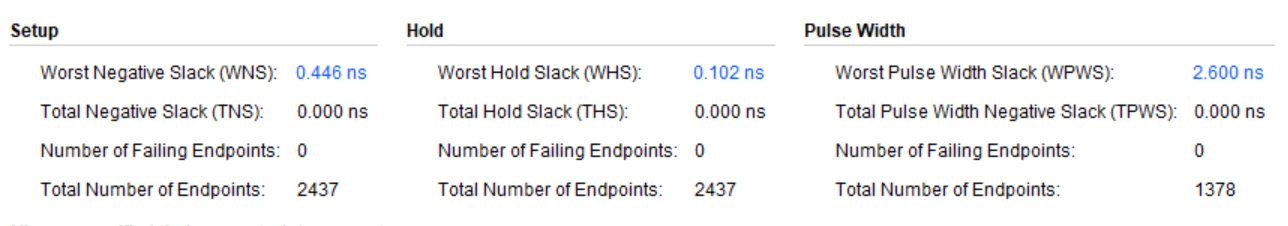
\includegraphics[width=0.92\textwidth]{figures/时序分析.png}
    \caption{Vivado 时序分析总览截图}
    \label{fig:timing_summary}
\end{figure}

\begin{table}[H]
    \centering
    \caption{时序分析总览}
    \label{tab:timing_summary}
    \begin{tabular}{lrrl}
        \toprule
        类型 & 违例端点数 & 最坏松弛（WNS/WHS/WPWS） & 总违例量 \\
        \midrule
        建立时间（Setup） & \textbf{0} & $+$0.446\,ns & 0.000\,ns \\
        保持时间（Hold）  & \textbf{0} & $+$0.102\,ns & 0.000\,ns \\
        脉冲宽度（PW）    & \textbf{0} & $+$2.600\,ns & 0.000\,ns \\
        \midrule
        \multicolumn{2}{l}{总端点数} & \multicolumn{2}{l}{2437（Setup/Hold），1378（PW）} \\
        \bottomrule
    \end{tabular}
\end{table}

结论：\textbf{建立时间、保持时间和脉冲宽度均满足，设计在 6\,ns（167\,MHz）约束下零违例}。
根据最坏建立时间松弛，可实现的最高频率估算为：

\begin{equation}
    F_{\max} \approx \frac{1}{T_{\text{constraint}} - \text{WNS}} = \frac{1}{6.000 - 0.446}\,\text{ns} = \frac{1}{5.554\,\text{ns}} \approx \mathbf{180\,MHz}
\end{equation}

\subsection{资源利用率}

综合后资源利用率如\autoref{fig:resource}和\autoref{tab:resource}所示，整个处理器仅占用 Virtex-7 极小比例资源。

\begin{figure}[H]
    \centering
    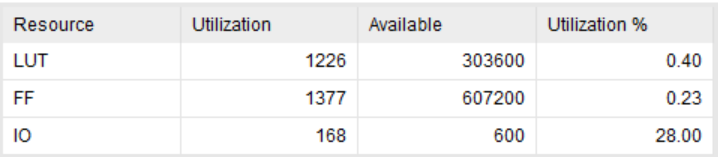
\includegraphics[width=0.72\textwidth]{figures/资源利用率.png}
    \caption{Vivado 资源利用率截图}
    \label{fig:resource}
\end{figure}

\begin{table}[H]
    \centering
    \caption{综合资源利用率}
    \label{tab:resource}
    \begin{tabular}{lrrr}
        \toprule
        资源类型 & 使用量 & 可用量 & 占用率 \\
        \midrule
        LUT（查找表） & 1\,226 & 303\,600 & 0.40\% \\
        FF（触发器）  & 1\,377 & 607\,200 & 0.23\% \\
        IO（引脚）    &   168  &     600  & 28.00\% \\
        \bottomrule
    \end{tabular}
\end{table}

LUT 用于组合逻辑（译码、ALU、转发选择、分支判断等），FF 对应流水线寄存器和通用寄存器堆（32×32 bit = 1024 个触发器）。IO 占比相对较高（28\%）是因为处理器顶层直接暴露了指令/数据总线的所有位宽端口。

\subsection{关键路径分析}

最差建立时间路径如\autoref{fig:worst_path}所示，详情见\autoref{tab:crit_path}。

\begin{figure}[H]
    \centering
    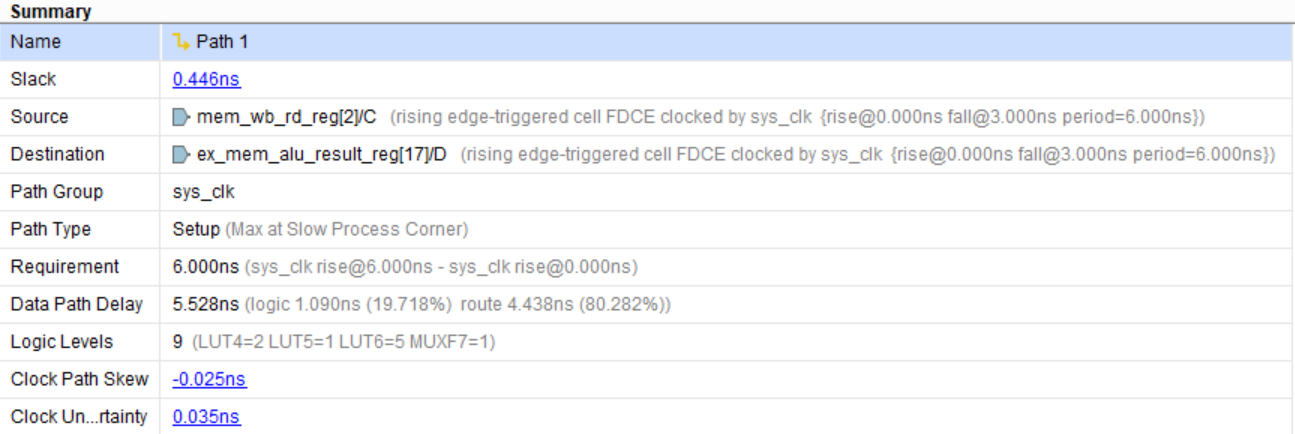
\includegraphics[width=0.98\textwidth]{figures/最差路径.png}
    \caption{Vivado 最差关键路径截图（WNS = $+$0.446\,ns）}
    \label{fig:worst_path}
\end{figure}

\begin{table}[H]
    \centering
    \caption{最差关键路径详情}
    \label{tab:crit_path}
    \begin{tabular}{ll}
        \toprule
        属性 & 值 \\
        \midrule
        路径类型 & Setup（建立时间，Slow Corner） \\
        松弛（Slack） & $+$0.446\,ns（满足） \\
        时钟约束（Requirement） & 6.000\,ns \\
        数据路径总延迟 & 5.528\,ns \\
        \quad 逻辑延迟（Logic） & 1.090\,ns（19.7\%） \\
        \quad 布线延迟（Route） & 4.438\,ns（80.3\%） \\
        逻辑级数 & 9（LUT4$\times$2，LUT5$\times$1，LUT6$\times$5，MUXF7$\times$1） \\
        时钟路径偏斜 & $-$0.025\,ns \\
        时钟不确定性 & 0.035\,ns \\
        起始节点（Source） & \texttt{mem\_wb\_rd\_reg[2]/C}（MEM/WB 寄存器，目标寄存器地址位 2） \\
        终止节点（Dest）   & \texttt{ex\_mem\_alu\_result\_reg[17]/D}（EX/MEM 寄存器，ALU 结果位 17） \\
        \bottomrule
    \end{tabular}
\end{table}

\subsection{关键路径根因分析}

关键路径从 \textbf{MEM/WB 流水线寄存器}的目标寄存器地址字段（\texttt{mem\_wb\_rd\_reg[2]}）出发，经过 9 级组合逻辑，落点于 \textbf{EX/MEM 流水线寄存器}的 ALU 结果字段（\texttt{ex\_mem\_alu\_result\_reg[17]}）。路径形成机制如下：

\begin{enumerate}[leftmargin=2em]
    \item \textbf{转发比较逻辑}：EX 阶段数据转发检测需将 \texttt{mem\_wb\_rd} 与 \texttt{id\_ex\_rs1}/\texttt{id\_ex\_rs2} 进行相等比较，产生转发使能信号（约 2--3 级 LUT）；
    \item \textbf{转发多路选择器}：根据比较结果，在 \texttt{wb\_data}、\texttt{ex\_mem\_alu\_result} 和 \texttt{id\_ex\_rdata1} 三路之间选择 EX 操作数（MUXF7 + 若干 LUT6）；
    \item \textbf{ALU 运算}：选定的操作数经过 ALU 组合逻辑（加法器、移位等）计算最终结果，多位进位链进一步增加了级数；
    \item \textbf{写入 EX/MEM 寄存器}：ALU 结果在时钟上升沿锁存到 \texttt{ex\_mem\_alu\_result\_reg}。
\end{enumerate}

本质原因是：\textbf{距离 2 拍的 MEM/WB$\rightarrow$EX 转发路径串联了「rd 比较 $\rightarrow$ 多路选择 $\rightarrow$ ALU 计算」三段逻辑，共产生约 5.5\,ns 的组合延迟}。布线延迟占比 80.3\% 说明 MEM/WB 寄存器与 EX 阶段逻辑在芯片上物理距离较远，若通过 \texttt{Pblock} 约束将两者归约至相邻区域，布线延迟可显著压缩，进一步提高 $F_{\max}$。

\subsection{优化建议}

\begin{table}[H]
    \centering
    \caption{时序优化方案对比}
    \label{tab:optimizations}
    \begin{tabular}{lp{5.2cm}ll}
        \toprule
        方案 & 具体做法 & 预期效果 & 代价 \\
        \midrule
        提高时钟频率 & 将约束从 6\,ns 收紧至 5.6\,ns（$\approx$180\,MHz） & 仍无违例（余量 0.446\,ns） & 近乎无代价 \\
        Pblock 布局约束 & 约束 EX 阶段与 MEM/WB 寄存器物理相邻 & 布线延迟从 4.4\,ns 降至约 2\,ns & 需掌握 Vivado 布局约束语法 \\
        流水线 WB 寄存前移 & 在 MEM/WB 与 EX 之间增加一级寄存，使转发数据提前一拍稳定 & 彻底断开长链路 & 增加 1 拍流水延迟，写回更晚 \\
        减少转发优先级级联 & 将三路转发合并为优先级编码，减少多路选择器深度 & 减少约 1--2 级 LUT & 需修改转发逻辑结构 \\
        \bottomrule
    \end{tabular}
\end{table}

当前设计已满足 6\,ns 约束，\textbf{最简单的下一步优化是将约束收紧至 5.6\,ns（180\,MHz）}，利用现有 0.446\,ns 余量验证是否仍无违例，无需修改任何 RTL 代码。

% =======================================================
\section{选做一：RV32I 完整指令集补全}
% =======================================================

\subsection{补全目标}

基础实验仅实现 13 条指令。本节在单周期（\texttt{single/}）与流水线（\texttt{pipeline/}）两种处理器上，补全了 RV32I 整数基础指令集中的剩余主要指令，新增 21 条，涵盖比较、算术移位、字节/半字访存、全部分支、LUI/AUIPC 和 JALR，详见\autoref{tab:new_isa}。

\begin{table}[H]
    \centering
    \caption{新增 RV32I 指令一览}
    \label{tab:new_isa}
    \begin{tabular}{>{\centering}p{1.4cm} >{\centering}p{1.3cm} c >{\centering}p{5cm} c}
        \toprule
        类别 & 指令 & 格式 & 功能描述 & ALU 操作码 \\
        \midrule
        \multirow{3}{*}{比较} & SLT   & R & $\text{rd}=(\text{rs1}<_s\text{rs2})\,?\,1:0$（有符号） & 4'd7 \\
                               & SLTU  & R & $\text{rd}=(\text{rs1}<_u\text{rs2})\,?\,1:0$（无符号） & 4'd8 \\
                               & SLTI  & I & $\text{rd}=(\text{rs1}<_s\text{imm})\,?\,1:0$ & 4'd7 \\
                               & SLTIU & I & $\text{rd}=(\text{rs1}<_u\text{imm})\,?\,1:0$ & 4'd8 \\
        \midrule
        移位 & SRA   & R & $\text{rd}=\text{rs1}\gg_a\text{rs2}[4:0]$（算术右移） & 4'd9 \\
              & SRAI  & I & $\text{rd}=\text{rs1}\gg_a\text{imm}[4:0]$ & 4'd9 \\
        \midrule
        \multirow{4}{*}{Load} & LB  & I & $\text{rd}=\text{sign\_ext}(\text{Mem}[\text{addr}][7:0])$ & 4'd0 \\
                               & LH  & I & $\text{rd}=\text{sign\_ext}(\text{Mem}[\text{addr}][15:0])$ & 4'd0 \\
                               & LBU & I & $\text{rd}=\text{zero\_ext}(\text{Mem}[\text{addr}][7:0])$ & 4'd0 \\
                               & LHU & I & $\text{rd}=\text{zero\_ext}(\text{Mem}[\text{addr}][15:0])$ & 4'd0 \\
        \midrule
        \multirow{2}{*}{Store} & SB & S & $\text{Mem}[\text{addr}][7:0]=\text{rs2}[7:0]$ & 4'd0 \\
                                & SH & S & $\text{Mem}[\text{addr}][15:0]=\text{rs2}[15:0]$ & 4'd0 \\
        \midrule
        \multirow{4}{*}{分支} & BNE  & B & if (rs1$\neq$rs2) PC$\mathrel{+}=$imm & 4'd1 \\
                               & BGE  & B & if (rs1$\geq_s$rs2) PC$\mathrel{+}=$imm（有符号） & 4'd7 \\
                               & BLTU & B & if (rs1$<_u$rs2) PC$\mathrel{+}=$imm（无符号） & 4'd8 \\
                               & BGEU & B & if (rs1$\geq_u$rs2) PC$\mathrel{+}=$imm & 4'd8 \\
        \midrule
        \multirow{2}{*}{立即数} & LUI   & U & $\text{rd}=\text{imm}_{u}$（高 20 位） & 4'd0 \\
                                 & AUIPC & U & $\text{rd}=\text{PC}+\text{imm}_{u}$ & 4'd0 \\
        \midrule
        跳转 & JALR & I & $\text{rd}=\text{PC}+4;\ \text{PC}=(\text{rs1}+\text{imm})\&{\sim}1$ & 4'd0 \\
        \bottomrule
    \end{tabular}
\end{table}

\subsection{各模块改动要点}

\subsubsection{ALU 新增运算（\texttt{ex.v}，单周期与流水线相同）}

在 \texttt{case(alu\_op)} 中新增三个操作码：

\begin{lstlisting}[caption={ALU 新增运算（SLT/SLTU/SRA）}]
4'd7: alu_result = ($signed(src1) < $signed(src2)) ? 32'd1 : 32'd0; // SLT
4'd8: alu_result = (src1 < src2) ? 32'd1 : 32'd0;                   // SLTU
4'd9: alu_result = $signed(src1) >>> src2[4:0];                      // SRA
\end{lstlisting}

有符号比较使用 \texttt{\$signed()} 强制转换，无符号比较直接用 \texttt{<}（Verilog 默认无符号语义）。

\subsubsection{ID 译码器扩展（\texttt{id.v}）}

\paragraph{新增输出信号}

\begin{itemize}[leftmargin=2em]
    \item \textbf{单周期}：新增 \texttt{load\_func3[2:0]} 和 \texttt{store\_func3[2:0]}，分别传递 func3 字段至 MEM 阶段，用于区分字节/半字/字访存。
    \item \textbf{流水线}：在上述基础上，还新增 \texttt{branch\_type[2:0]}（扩展自 2 位）、\texttt{jalr}、\texttt{write\_pc4}，将分支解析移至 EX 阶段。
\end{itemize}

\paragraph{LUI 与 AUIPC}

LUI 需将高 20 位立即数 \texttt{imm\_u} 直接载入目标寄存器。实现方案：强制 \texttt{rs1=5'b0}，使寄存器堆读出 0，再令 ALU 计算 $0 + \text{imm\_u} = \text{imm\_u}$。

\begin{lstlisting}[caption={LUI/AUIPC 译码（以流水线 id.v 为例）}]
7'b0110111: begin  // LUI
    rs1=5'b0; rs2=5'b0; reg_we=1; src1_sel=0; src2_sel=2'd1;
    alu_op=4'd0; imm=imm_u;  // ALU: 0 + imm_u = imm_u
end
7'b0010111: begin  // AUIPC
    rs1=5'b0; rs2=5'b0; reg_we=1; src1_sel=1; src2_sel=2'd1;
    alu_op=4'd0; imm=imm_u;  // ALU: PC + imm_u
end
\end{lstlisting}

\paragraph{条件分支扩展}

BLT/BGE 使用 SLT（操作码 7）而非减法来判断有符号大小关系，可避免有符号溢出（如 $\text{INT\_MIN} - 1$ 会上溢导致减法符号位错误）。BLTU/BGEU 类似，使用 SLTU（操作码 8）。流水线版 \texttt{branch\_type} 编码如\autoref{tab:branch_type}所示。

\begin{table}[H]
    \centering
    \caption{流水线 branch\_type 编码与对应 ALU 操作}
    \label{tab:branch_type}
    \begin{tabular}{cclcc}
        \toprule
        branch\_type & 指令 & 跳转条件 & ALU 操作 & 跳转判定 \\
        \midrule
        3'd0 & — & 无分支 & — & — \\
        3'd1 & BEQ  & rs1 = rs2 & SUB（4'd1） & alu\_result = 0 \\
        3'd2 & BNE  & rs1 $\neq$ rs2 & SUB（4'd1） & alu\_result $\neq$ 0 \\
        3'd3 & BLT  & rs1 $<_s$ rs2 & SLT（4'd7） & alu\_result = 1 \\
        3'd4 & BGE  & rs1 $\geq_s$ rs2 & SLT（4'd7） & alu\_result = 0 \\
        3'd5 & BLTU & rs1 $<_u$ rs2 & SLTU（4'd8） & alu\_result = 1 \\
        3'd6 & BGEU & rs1 $\geq_u$ rs2 & SLTU（4'd8） & alu\_result = 0 \\
        \bottomrule
    \end{tabular}
\end{table}

\paragraph{JALR}

JALR 的跳转目标（$\text{rs1}+\text{imm}$）在 EX 阶段才能确定（需要转发后的 rs1）。两种处理器实现策略不同：
\begin{itemize}[leftmargin=2em]
    \item \textbf{单周期}：ID 阶段直接读 \texttt{rdata1}（无转发问题），计算 \texttt{next\_pc=(rdata1+imm\_i)\&\textasciitilde 1}，同时令 ALU 计算 PC+4 作为返回地址写入 \texttt{rd}。
    \item \textbf{流水线}：设置 \texttt{jalr=1} 传至 ID/EX，令 ALU 计算 \texttt{rs1+imm}（目标地址），EX 阶段发现 \texttt{id\_ex\_jalr=1} 即触发跳转；写回地址通过 \texttt{write\_pc4=1} 标志传递，WB 写回 \texttt{id\_ex\_pc+4}。
\end{itemize}

\subsubsection{字节/半字访存（\texttt{mem.v}，单周期与流水线相同）}

数据存储器 \texttt{data\_mem.v} 为字节寻址（\texttt{addr} 直接作为字节地址），且提供独立的字节写使能 \texttt{we[3:0]}。\texttt{mem\_stage} 根据 \texttt{store\_func3} 和 \texttt{load\_func3} 生成正确的字节使能与数据提取逻辑：

\begin{lstlisting}[caption={字节写使能生成（STORE）}]
if (mem_we == 4'b1111 && mem_ce) begin
    case (store_func3[1:0])
        2'b00: mem_we_o = 4'b0001;   // SB：仅最低字节
        2'b01: mem_we_o = 4'b0011;   // SH：低两字节
        default: mem_we_o = 4'b1111; // SW：全字
    endcase
end
\end{lstlisting}

\begin{lstlisting}[caption={加载数据提取（LOAD）}]
case (load_func3)
    3'b000: load_data = {{24{rdata[7]}},  rdata[7:0]};   // LB：符号扩展字节
    3'b001: load_data = {{16{rdata[15]}}, rdata[15:0]};  // LH：符号扩展半字
    3'b010: load_data = rdata;                             // LW：全字
    3'b100: load_data = {24'b0, rdata[7:0]};              // LBU：零扩展字节
    3'b101: load_data = {16'b0, rdata[15:0]};             // LHU：零扩展半字
endcase
\end{lstlisting}

\subsubsection{流水线顶层重构（\texttt{pipeline/riscv.v}）}

流水线顶层需要针对新增指令进行较大改动，主要包括：

\paragraph{新增流水线寄存器字段}

ID/EX 新增：\texttt{id\_ex\_branch\_type[2:0]}、\texttt{id\_ex\_jalr}、\texttt{id\_ex\_write\_pc4}、\\
\texttt{id\_ex\_load\_func3[2:0]}、\texttt{id\_ex\_store\_func3[2:0]}。\\
EX/MEM 新增：\texttt{ex\_mem\_load\_func3}、\texttt{ex\_mem\_store\_func3}、\texttt{ex\_mem\_write\_pc4}、\texttt{ex\_mem\_return\_pc}（JALR 返回地址）。\\
MEM/WB 新增：\texttt{mem\_wb\_write\_pc4}、\texttt{mem\_wb\_return\_pc}。

\paragraph{EX 阶段分支/JALR 解析}

条件分支和 JALR 的跳转均在 EX 阶段判断（此时转发已稳定），产生 \texttt{ex\_branch\_taken} 和 \texttt{ex\_branch\_target}，并冲刷 IF/ID 和 ID/EX 两级（2 拍损失）：

\begin{lstlisting}[caption={EX 阶段分支解析与 JALR 跳转}]
assign ex_branch_taken =
    (id_ex_branch_type==3'd1 && alu_result==32'd0)  ||  // BEQ
    (id_ex_branch_type==3'd2 && alu_result!=32'd0)  ||  // BNE
    (id_ex_branch_type==3'd3 && alu_result==32'd1)  ||  // BLT
    (id_ex_branch_type==3'd4 && alu_result==32'd0)  ||  // BGE
    (id_ex_branch_type==3'd5 && alu_result==32'd1)  ||  // BLTU
    (id_ex_branch_type==3'd6 && alu_result==32'd0)  ||  // BGEU
    id_ex_jalr;

assign ex_branch_target = id_ex_jalr ?
    (alu_result & ~32'h1) :      // JALR：(rs1+imm) & ~1
    (id_ex_pc  + id_ex_imm);     // 条件分支：PC + imm_b
\end{lstlisting}

\paragraph{JALR 写回（\texttt{write\_pc4} 传递链）}

JALR 写回的是 PC+4 而非 ALU 结果，通过 \texttt{write\_pc4} 标志沿流水线传递，在 WB 选择写回数据时最高优先级选择 \texttt{return\_pc}：

\begin{lstlisting}[caption={WB 写回数据选择（含 JALR）}]
assign wb_data = mem_wb_write_pc4                             ? mem_wb_return_pc  :
                 (mem_wb_mem_we == 4'b0 && mem_wb_mem_ce)    ? mem_wb_load_data  :
                                                                mem_wb_alu_result ;
\end{lstlisting}

\subsection{测试程序设计与验证}

\subsubsection{测试策略}

新编写 40 条指令的汇编测试程序（机器码写入 \texttt{machinecode.txt}），按序覆盖全部新增指令类型，最终将通过次数计数器 \texttt{x9} 通过 \texttt{SW x9, 12(x0)} 写入 \texttt{verify} 地址（字节地址 12），预期值为 \textbf{6}。

\subsubsection{测试程序流程}

\begin{enumerate}[leftmargin=2em]
    \item \textbf{算术/比较/移位}（指令 0--7）：验证 SLT、SLTU、SRA、SLTI、SLTIU、LUI。\\
          $\text{x1}=-1$，$\text{x2}=1$：$\text{SLT}\Rightarrow\text{x3}=1$；$\text{SLTU}\Rightarrow\text{x4}=0$；$\text{SRA}\Rightarrow\text{x5}=-1$；\\
          $\text{SLTI x6, x1, 0}\Rightarrow\text{x6}=1$（$-1<0$）；$\text{SLTIU x7, x0, 1}\Rightarrow\text{x7}=1$（$0<1$）；\\
          $\text{LUI x8, 0xDEADB}\Rightarrow\text{x8}=\texttt{0xDEADB000}$。

    \item \textbf{分支测试}（指令 8--23）：依次测试 BNE、BLT、BGE、BLTU、BGEU，每条分支均设计为应跳转，跳过 1 条 NOP，落入 \texttt{ADDI x9, x9, 1}。全部跳转正确则 $\text{x9}=5$。

    \item \textbf{字节/半字访存}（指令 24--31）：\\
          SB + LB（预期 $\text{x11}=\texttt{0xFFFFFFFF}$，符号扩展 0xFF）；\\
          LBU（预期 $\text{x12}=\texttt{0x000000FF}$，零扩展）；\\
          SH + LH（预期 $\text{x14}=\texttt{0xFFFFFFFF}$）；\\
          LHU（预期 $\text{x15}=\texttt{0x0000FFFF}$）。

    \item \textbf{AUIPC + JALR}（指令 32--37）：\\
          \texttt{AUIPC x16, 0}$\Rightarrow\text{x16}=128$（当前 PC）；\\
          \texttt{JALR x17, x16, 20}$\Rightarrow$跳转至 $128+20=148$，跳过 3 条 NOP，\\
          落入 \texttt{ADDI x9, x9, 1}$\Rightarrow\text{x9}=6$。

    \item \textbf{写入验证值}（指令 38）：\texttt{SW x9, 12(x0)} $\Rightarrow$ \texttt{verify} = 6。

    \item \textbf{无限循环}（指令 39）：\texttt{JAL x0, 0}，防止 PC 越界。
\end{enumerate}

\subsubsection{验证结果}

仿真输出：
\begin{center}
\texttt{---\quad result is \textbf{6}\quad ---}
\end{center}

单周期与流水线处理器均输出 \texttt{verify = 6}，与预期一致，证明新增 21 条指令的功能均正确。

% =======================================================
\section{选做二：自由拓展——AI 辅助开发}
% =======================================================

\subsection{概述}

本次实验的选做内容（RV32I 指令集补全）采用了 AI 辅助开发的工作流程，借助 Claude AI 大语言模型协助进行架构设计、代码生成与验证，最终显著提升了设计迭代效率。

\subsection{AI 辅助内容}

\subsubsection{架构设计决策}

在扩展流水线支持全 RV32I 时，存在多个关键设计抉择，由 AI 协助分析权衡：

\begin{itemize}[leftmargin=2em]
    \item \textbf{条件分支在哪个阶段解析}：单周期可在 ID 阶段直接使用 \texttt{rdata1/rdata2} 比较，但流水线若在 ID 解析，遇到数据相关时需等到转发完成，反而增加阻塞。AI 分析后建议：\textbf{流水线分支移至 EX 阶段}——利用 EX 阶段已完成的转发值进行比较，代价仅多冲刷 1 拍（共 2 拍），逻辑更清晰。

    \item \textbf{BLT/BGE 使用减法还是 SLT 判断}：使用减法（\texttt{rs1-rs2}）检查符号位会在 $\text{rs1}>0, \text{rs2}<0$ 时因有符号溢出产生错误结果。AI 指出应直接使用 SLT ALU 操作（操作码 7），其内部用 \texttt{\$signed} 比较，避免溢出陷阱。

    \item \textbf{JALR 返回地址路径}：ALU 被占用于计算目标地址（\texttt{rs1+imm}），返回地址 \texttt{PC+4} 需要单独传递。AI 建议引入 \texttt{write\_pc4} 标志沿流水线传递，WB 阶段优先写回 \texttt{id\_ex\_pc+4}，与 LOAD 路径并行存在，避免额外 ALU 占用。

    \item \textbf{距离 3 拍 RAW 与写优先}：在以 250\,MHz（4\,ns）时钟进行的初步综合中，Vivado 报告了 WNS = $-2.301$\,ns 的建立时间违例，关键路径为「寄存器堆读 $\rightarrow$ ID 阶段组合 $\rightarrow$ 写优先选择 $\rightarrow$ 寄存器堆写」长链（9 级 LUT，近 6\,ns）。AI 定位到根本原因是 \texttt{register.v} 中的写优先（Write-First）组合逻辑，建议将其替换为 ID/EX 捕获转发（在 ID/EX 寄存器锁存时直接注入 \texttt{wb\_data}），以断开跨 WB$\to$ID$\to$写的组合链。优化后以 6\,ns（167\,MHz）约束重新综合，设计全部满足时序（WNS = $+$0.446\,ns，零违例），关键路径缩短为 MEM/WB 转发 $\rightarrow$ EX ALU 路径（5.528\,ns）。
\end{itemize}

\subsubsection{代码生成与审查}

AI 生成了以下模块的完整 Verilog 代码并逐行说明设计意图：

\begin{itemize}[leftmargin=2em]
    \item \texttt{ex.v}（单周期 + 流水线）：新增 SLT/SLTU/SRA 的 ALU case 分支；
    \item \texttt{id.v}（单周期）：全 RV32I 组合译码逻辑，含 LUI/AUIPC/JALR 特殊操作数处理；
    \item \texttt{id.v}（流水线）：在单周期版基础上抽取分支类型编码，新增 \texttt{branch\_type[2:0]}、\texttt{jalr}、\texttt{write\_pc4} 输出；
    \item \texttt{mem.v}（单周期 + 流水线）：字节/半字 STORE 使能生成与 LOAD 数据提取；
    \item \texttt{riscv.v}（流水线顶层）：新增流水线寄存器字段、EX 阶段分支解析、双级冲刷逻辑、JALR 写回链路。
\end{itemize}

\subsubsection{测试程序生成}

AI 根据指令格式规范手工编码 40 条 RV32I 指令（\autoref{tab:machine_code}），涵盖所有新增指令类型，并以追踪变量 \texttt{x9} 的方式设计可自动验证的测试策略（最终 \texttt{verify=6} 表示全部 5 个分支均正确跳转，JALR 也正确执行）。

\begin{table}[H]
    \centering
    \caption{测试程序机器码节选}
    \label{tab:machine_code}
    \begin{tabular}{llll}
        \toprule
        机器码 & 汇编指令 & 预期结果 & 测试项 \\
        \midrule
        \texttt{FFF00093} & \texttt{addi x1, x0, -1}  & x1=0xFFFFFFFF & 初始化 \\
        \texttt{0020A1B3} & \texttt{slt x3, x1, x2}   & x3=1          & SLT \\
        \texttt{0020B233} & \texttt{sltu x4, x1, x2}  & x4=0          & SLTU \\
        \texttt{4020D2B3} & \texttt{sra x5, x1, x2}   & x5=0xFFFFFFFF & SRA \\
        \texttt{DEADB437} & \texttt{lui x8, 0xDEADB}  & x8=0xDEADB000 & LUI \\
        \texttt{00209463} & \texttt{bne x1, x2, +8}   & 跳转，x9+1   & BNE \\
        \texttt{0020C463} & \texttt{blt x1, x2, +8}   & 跳转，x9+1   & BLT \\
        \texttt{00115463} & \texttt{bge x2, x1, +8}   & 跳转，x9+1   & BGE \\
        \texttt{00106463} & \texttt{bltu x0, x1, +8}  & 跳转，x9+1   & BLTU \\
        \texttt{0000F463} & \texttt{bgeu x1, x0, +8}  & 跳转，x9+1   & BGEU \\
        \texttt{00A00023} & \texttt{sb x10, 0(x0)}    & Mem[0]=0xFF   & SB \\
        \texttt{00000583} & \texttt{lb x11, 0(x0)}    & x11=0xFFFFFFFF& LB \\
        \texttt{00004603} & \texttt{lbu x12, 0(x0)}   & x12=0xFF      & LBU \\
        \texttt{00000817} & \texttt{auipc x16, 0}     & x16=PC=128    & AUIPC \\
        \texttt{01480867} & \texttt{jalr x17,x16,20}  & 跳转至 148    & JALR \\
        \texttt{00902623} & \texttt{sw x9, 12(x0)}    & verify=6      & 验证写回 \\
        \bottomrule
    \end{tabular}
\end{table}

\subsection{AI 辅助开发体会}

\begin{itemize}[leftmargin=2em]
    \item \textbf{缩短迭代周期}：相比纯手工设计，AI 能快速给出详细的比特级编码计算和信号路径追踪，避免了在规范文档中反复查找位域定义的时间损耗，单个模块的设计-验证周期从数小时压缩至十几分钟。

    \item \textbf{问题诊断辅助}：当流水线 BEQ/BLT 在仿真中始终不跳转时，AI 通过分析原始 \texttt{riscv.v} 源代码，快速定位到 \texttt{branch\_type} 信号在顶层虽已声明但从未被连接至 EX 阶段逻辑的根本原因，节省了大量调试时间。

    \item \textbf{局限性}：AI 不能替代真实的仿真工具，复杂冲突场景（如 Load-Use + 分支同时发生）仍需通过 QuestaSim 波形进行最终验证。AI 生成的代码也需要人工审查，确保符合实际硬件语义（如非阻塞赋值的使用、always 块敏感列表等）。

    \item \textbf{合规性说明}：本实验所有 AI 辅助均在实验规范允许的范围内进行（实验说明书明确将 AI 辅助开发列为自由拓展选项之一），所有生成代码均经本人理解、审查和修改后方才采用。
\end{itemize}

% =======================================================
\section{总结}
% =======================================================

\subsection{设计总结}

本实验在基础实验的 13 条指令基础上，通过选做内容进一步补全了完整 RV32I 指令集，主要完成内容如下：

\begin{enumerate}[leftmargin=2em]
    \item \textbf{单周期处理器}：建立 IF--ID--EX--MEM--WB 五阶段组合逻辑数据通路，在 ID 阶段完成分支条件计算与 PC 控制，实现了 RV32I 主要指令的零缺陷执行。代码备份于 \texttt{single/} 目录。

    \item \textbf{流水线改造}：在单周期基础上于级间插入 4 组流水线寄存器，构建五级流水线结构；实现三条数据转发路径（EX/MEM$\rightarrow$EX、MEM/WB$\rightarrow$EX、ID/EX 捕获转发）解决 RAW 冲突；Load-Use 冲突通过 \texttt{stall\_req} 机制暂停 1 拍处理；控制冲突通过冲刷 IF/ID 和 ID/EX 两级处理（JAL 冲刷 1 拍，条件分支/JALR 冲刷 2 拍）。

    \item \textbf{RV32I 指令集补全（选做）}：在两种处理器上新增 21 条指令，涵盖 SLT/SLTU/SRA、字节/半字访存（LB/LH/LBU/LHU/SB/SH）、全部分支（BNE/BGE/BLTU/BGEU）、LUI/AUIPC/JALR；编写了 40 条指令的自动化验证测试程序，仿真验证两种处理器均输出预期结果 \texttt{verify = 6}。

    \item \textbf{AI 辅助开发（选做）}：借助 Claude AI 大语言模型协助架构决策、代码生成与测试程序编码，并在实验报告中如实记录了 AI 辅助的范围与局限性。
\end{enumerate}

\subsection{性能分析}

\begin{table}[H]
    \centering
    \caption{单周期与五级流水线处理器性能对比}
    \label{tab:perf_compare}
    \begin{tabular}{lll}
        \toprule
        指标 & 单周期 & 五级流水线 \\
        \midrule
        时钟周期约束 & 最长路径（含 LW 全通路） & 最长\emph{单阶段}路径（约 1/5） \\
        理论最高频率 & 低（~100 MHz 量级） & 高（约 5$\times$，~500 MHz 量级） \\
        理想 CPI & 1 & 趋近 1 \\
        Load-Use 代价 & 无（固定 1 周期/指令） & +1 周期/发生 \\
        Branch 代价 & 无 & +1 周期/发生 \\
        实际吞吐量 & 低 & 高（频率提升远大于冲突损失） \\
        设计复杂度 & 低 & 高（需处理三类冲突） \\
        \bottomrule
    \end{tabular}
\end{table}

\subsection{心得体会}

通过本次实验，对流水线处理器设计的核心难点有了切身体会：

\begin{itemize}[leftmargin=2em]
    \item \textbf{数据相关无处不在}：从单周期改为流水线的第一步便要系统梳理所有可能的写后读场景，距离 1/2/3 拍的处理策略各有差异，不可遗漏。

    \item \textbf{Load-Use 的特殊性}：LW 的结果在 MEM 阶段末才就绪，是流水线中唯一无法靠纯转发消除的 RAW 冲突，必须引入暂停机制，这也是通常 LW 后需要编译器主动插入独立指令以隐藏延迟的原因。

    \item \textbf{控制信号也需打拍}：流水线寄存器不仅要传递数据（rdata1/2、imm、PC），还需携带与数据对齐的控制信号（reg\_we、mem\_ce、mem\_we 等），确保在正确的阶段发出正确的控制。

    \item \textbf{JAL 的操作数特殊性}：JAL 需要以 PC 作为 src1，而 PC 不在寄存器堆中，必须在 ID/EX 寄存器中单独传递 PC 并引入 \texttt{src1\_sel} 信号，这是将单周期直接复用为流水线子模块时容易忽略的细节。
\end{itemize}

\end{document}
